\documentclass{beamer}

\usepackage{hyperref}
\usepackage{graphicx}

\title{MATH 1190 \& 1210 Meeting for Week 6}
\author{Josh}
\date{16 February 2026}

\newcommand{\transition}[1]{\frame{{}\begin{center}\fbox{#1}\end{center}}}

\begin{document}

\maketitle
\section*{Logistics}

\transition{Logistics}
%------------------------------------------------
\begin{frame}{Upcoming Schedule}
\begin{itemize}
    \item This week (Week 6): Lessons 9 and 10
    \item Exponential and log functions plus derivatives of exponential and log functions.
    \item Next week (Week 7): Lessons 11 and 12
    \item Local Extrema and First Derivative Tests Second Derivative Tests
    \item Week 8 is Spring Break and Assessment 2 is on Tuesday, March 9 the week after.
    \item Would like to make HW 12 due on Monday, March 9 so students can get practice, but I am worried about all sections getting to Lesson 12 before Tuesday.
\end{itemize}
\end{frame}
%------------------------------------------------

\section{Lessons}

\transition{Lessons}


%------------------------------------------------
\begin{frame}{Important Ideas: Lesson 9}
\paragraph{Lesson Goals} related to target {\bf\color{ProcessBlue} F2: Exponential \& Logarithmic Functions}
\begin{itemize}
    \item Apply the properties of exponents and logarithms to simplify an expression. 
    \item Find the values of logarithmic expressions.
    \item Know properties of exponential and logarithmic function to find their domain, range, and common limits.
    \item solve equations involving exponential and logarithmic functions.
\end{itemize}
\end{frame}

%------------------------------------------------
\begin{frame}{How the students are feeling}
{\it Specific feedback from Pre-Class:}
\begin{itemize}
\item ``I found it interesting that logs, which seem very difficult and abstract, are actually just exponents."
\item ``The beginning made a lot of sense since I learned this before, however, it got a little confusing pretty fast once we had to actually quickly calculate the logs/ln."
    \begin{itemize}
    \item DJ's note: some students may never have interacted with logarithms without a calculator before. So, these students may not really know how logarithms relate to exponents.
    \end{itemize}
\item ``Could you go over this problem in class from the last video? $\ln(e-1) + \ln(e^2+e) - \ln(e^4-e^2)$. I was confused on how to simplify it completely."
    \begin{itemize}
    \item DJ's note: this is the last task in the pre-class lesson, and exactly Example 3 in the in-class lesson.
    \end{itemize}
\end{itemize}
\end{frame}
%------------------------------------------------
\begin{frame}{Handout Structure — Flow of the Lesson}
\textbf{1. Exponent Foundations}
\begin{itemize}
    \item Example 1 → Model organized use of exponent rules.
    \item Exercise A → Immediate practice + common misconceptions:
    \begin{itemize}
        \item Radicals as fractional exponents
        \item Misuse of negative exponents
        \item “Freshman’s Dream”
    \end{itemize}
\end{itemize}

\bigskip

\textbf{2. Logs as Exponents}
\begin{itemize}
    \item Example 2 / Exercise B → Build inverse connection.
    \item Emphasize meaning over memorized tricks.
    \item Many students have little prior log exposure.
\end{itemize}

\bigskip

\textbf{3. Log Structure \& Condensing}
\begin{itemize}
    \item Example 3 / Exercise C → Combine first, simplify second.
    \item Physically reference log rules while modeling.
\end{itemize}
\end{frame}

%------------------------------------------------
\begin{frame}{Handout Structure — Conceptual Development}
\textbf{4. Function Understanding}
\begin{itemize}
    \item Exercises D \& E → Shape, domain, range.
    \item Reinforce inverse relationship visually.
    \item Encourage conjectures about derivatives (preview next lesson).
\end{itemize}

\bigskip

\textbf{5. Equation Solving \& Error Analysis}
\begin{itemize}
    \item Exercise F → Diagnose incorrect reasoning.
    \item Highlight:
    \begin{itemize}
        \item Same log on both sides
        \item No distributing exponentials
        \item Use log rules before exponentiating
    \end{itemize}
\end{itemize}

\bigskip

\textbf{6. Practice \& Extension}
\begin{itemize}
    \item Exam Practice → Students struggle most with simplification.
    \item Extra Practice 2 → See structural parallels between exponential and logarithmic equations.
    \item Final emphasis: structure over algorithm.
\end{itemize}
\end{frame}
%------------------------------------------------
\begin{frame}{Important Ideas: Lesson 10}
\paragraph{Lesson Goals} related to targets {\bf\color{ProcessBlue} D2 \& D3: Derivatives}

\begin{itemize}
    \item Derive and compute derivatives of general exponential functions, $a^x$.
    \item Derive and compute derivatives of general logarithmic functions, $\log_a(x)$.
    \item Use exponential and logarithmic derivatives within:
    \begin{itemize}
        \item Chain Rule
        \item Product Rule
        \item Quotient Rule
    \end{itemize}
    \item Decide which differentiation technique should be used to start.
    \item Apply these derivatives in context.
\end{itemize}
\end{frame}

%------------------------------------------------
\begin{frame}{Notes:}
\begin{itemize}
    \item No pre-class preparation → cognitive load may be higher.
    \item Students often:
    \begin{itemize}
        \item Memorize $e^x$ derivative but not $a^x$.
        \item Forget that $\ln(x)$ and $\log_a(x)$ are different.
        \item Struggle deciding how to start multi-rule problems.
    \end{itemize}
    \item Key struggle: identifying structure before differentiating.
\end{itemize}
\end{frame}

%------------------------------------------------
\begin{frame}{Handout Structure — Flow of the Lesson}
\textbf{1. Mini-Lecture: Derivative of $a^x$}
\begin{itemize}
    \item Emphasize derivation, not just formula.
    \item Highlight why $\ln(a)$ appears.
\end{itemize}

\bigskip

\textbf{2. Example 1 / Exercise A}
\begin{itemize}
    \item Practice with Chain Rule + $a^x$.
    \item Focus on: How do we decide how to begin?
    \item Identify structure:
    \begin{itemize}
        \item Function-within-a-function?
        \item Product?
        \item Quotient?
    \end{itemize}
\end{itemize}

\bigskip

\textbf{3. Exercise B (Context)}
\begin{itemize}
    \item Scaffolded applied problem.
    \item Identify parameters before differentiating.
\end{itemize}
\end{frame}

%------------------------------------------------
\begin{frame}{Handout Structure — Conceptual Development}
\textbf{4. Mini-Lecture: Derivative of $\log_a(x)$}
\begin{itemize}
    \item Connect to derivative of $\ln(x)$.
    \item Emphasize structure:
    \[
    \frac{d}{dx}\log_a(x) = \frac{1}{x\ln(a)}
    \]
    \item Show where $\ln(a)$ comes from.
\end{itemize}

\bigskip

\textbf{5. Exercises C \& D}
\begin{itemize}
    \item Practice combining:
    \begin{itemize}
        \item Log derivatives
        \item Chain Rule
        \item Product / Quotient Rules
    \end{itemize}
    \item Continue emphasizing: “What structure do you see first?”
\end{itemize}
\end{frame}

%------------------------------------------------
\begin{frame}{Practice \& Extension}
\textbf{Core Focus: Example 1, Exercises A--D}

\bigskip

\textbf{Discussion Question}
\begin{itemize}
    \item Strong conceptual opportunity if time allows.
\end{itemize}

\bigskip

\textbf{Extra Practice 1 \& 2}
\begin{itemize}
    \item Challenging multi-technique problems.
    \item Excellent for reinforcing decision-making at the start.
\end{itemize}

\bigskip

\textbf{Extra Practice 3}
\begin{itemize}
    \item In-context application.
\end{itemize}

\bigskip

\textbf{Final Emphasis:}
\begin{itemize}
    \item Structure recognition before computation.
    \item Technique selection is the main skill.
\end{itemize}
\end{frame}

%------------------------------------------------
\section{Pedagogy}

\transition{Pedagogy}
\section{Active Learning}

\transition{And Now - An Active Learning Discussion with Michael!}
%------------------------------------------------
%------------------------------------------------
\begin{frame}{Discussion}
\textbf{Xu (2024)}  
\textit{Student Engagement and Academic Achievement in Learning Calculus}  

\bigskip

\textbf{Purpose of Today}
\begin{itemize}
    \item Understand the study
    \item Evaluate its methodology and claims
    \item Consider implications for our calculus courses
\end{itemize}
\end{frame}

%------------------------------------------------
\begin{frame}{Study Purpose \& Research Question}
\textbf{Purpose:}
\begin{itemize}
    \item Examine the relationship between student engagement and achievement in university calculus.
\end{itemize}

\bigskip

\textbf{Research Question:}
\begin{itemize}
    \item Is there a statistically significant relationship between engagement and calculus achievement?
\end{itemize}

\bigskip

\textbf{Discussion}
\begin{itemize}
    \item Is this a question we assume we already know the answer to?
    \item Why might this question matter for lesson design?
\end{itemize}
\end{frame}

%------------------------------------------------
\begin{frame}{Conceptual Framework: What Is Engagement?}
\textbf{Engagement Dimensions:}
\begin{itemize}
    \item Behavioral
    \item Emotional
    \item Cognitive
\end{itemize}

\bigskip

Implicit assumption: Engagement $\rightarrow$ Achievement

\bigskip

\textbf{Discussion}
\begin{itemize}
    \item Which form of engagement do we prioritize in calculus?
    \item Do our classrooms visibly measure the kind of engagement that leads to understanding?
    \item Is “participation” a reliable proxy for learning?
\end{itemize}
\end{frame}

%------------------------------------------------

\begin{frame}{Theoretical Framework: Self-Determination Theory}
    \centering
    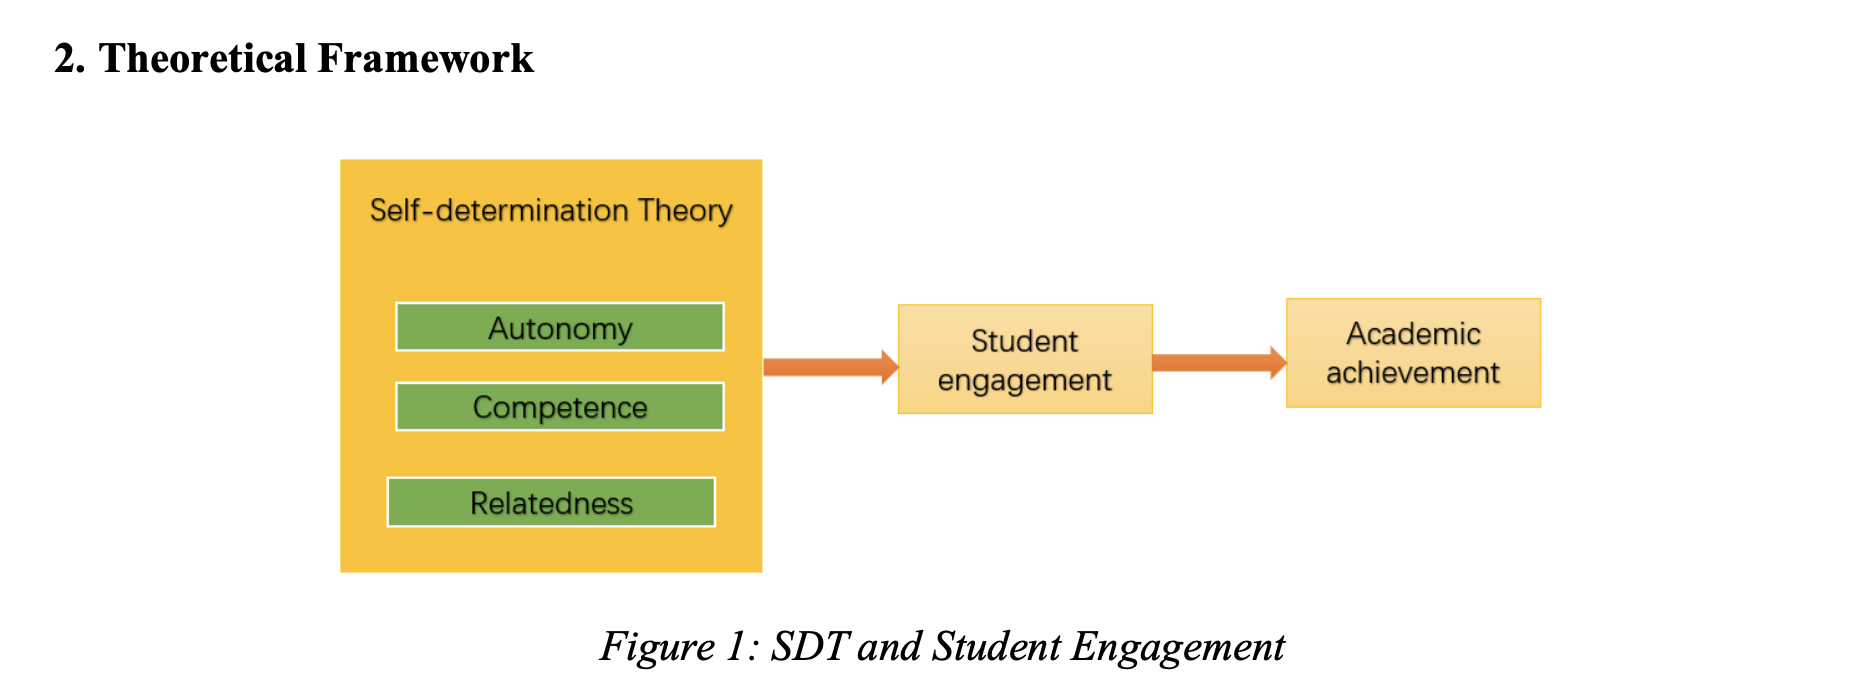
\includegraphics[width=0.9\textwidth]{SelfDetermiinationTheory.png}
\medskip
\small Graphic of Self-Determination Theory.
\end{frame}












\begin{frame}{Methodology}
\textbf{Design:}
\begin{itemize}
    \item Quantitative, correlational study
\end{itemize}

\textbf{Participants:}
\begin{itemize}
    \item Students in one university calculus course
\end{itemize}

\textbf{Data Sources:}
\begin{itemize}
    \item Engagement survey ("24 Questions "Agree", "Disagree", $\ldots$ numerical value assigned, mean taken)
    \item Course achievement scores
\end{itemize}

\bigskip

\textbf{Discussion}
\begin{itemize}
    \item What strengths do you see in this design?
    \item What important variables might be missing?
\end{itemize}
\end{frame}

%------------------------------------------------
\begin{frame}{Instrumentation}
\textbf{Engagement:}
\begin{itemize}
    \item Self-reported survey
    \item Multi-dimensional construct
\end{itemize}

\textbf{Achievement:}
\begin{itemize}
    \item Course grades
\end{itemize}

\bigskip

\textbf{Discussion}
\begin{itemize}
    \item Are grades an adequate measure of calculus understanding?
    \item What alternative measures might better capture achievement?
    \item How reliable is self-reported engagement?
\end{itemize}
\end{frame}

%------------------------------------------------
\begin{frame}{Data Analysis}
\textbf{Analysis Used:}
\begin{itemize}
    \item Descriptive statistics
    \item Pearson correlation
\end{itemize}

\bigskip

\textbf{Key Statistic:}
\begin{itemize}
    \item $r = 0.08$
    \item $p > 0.05$
    \item Pearson correlation coefficients:
        \begin{itemize}
            \item affective: 0.09
            \item behavioral: 0.09
            \item cognitive: 0.06
        \end{itemize}
\end{itemize}

\bigskip

No statistically significant relationship found.

\bigskip

\textbf{Discussion}
\begin{itemize}
    \item How should we interpret a near-zero correlation?
    \item Does absence of correlation imply absence of influence?
\end{itemize}
\end{frame}

%------------------------------------------------
\begin{frame}{Results and Interpretation}
\textbf{Findings:}
\begin{itemize}
    \item Students reported high engagement.
    \item Most achieved passing or strong grades.
    \item Engagement did not significantly predict achievement.
\end{itemize}

\bigskip

\textbf{Discussion}
\begin{itemize}
    \item What might explain this disconnect?
    \item Could engagement impact long-term retention rather than short-term grades?
    \item Does calculus assessment emphasize speed over depth?
\end{itemize}
\end{frame}

%------------------------------------------------
\begin{frame}{Limitations and Context}
\begin{itemize}
    \item Single institutional context
    \item Correlational (not causal)
    \item Self-reported engagement
    \item Achievement narrowly defined
\end{itemize}

\bigskip

\textbf{Discussion}
\begin{itemize}
    \item Would we expect similar results at UVA?
    \item How might class sizes affect outcomes?
    \item How could this study be redesigned in our context?
\end{itemize}
\end{frame}

%------------------------------------------------
\begin{frame}{Implications for Our Calculus Sequence}
If engagement does not automatically translate into achievement:

\begin{itemize}
    \item What kinds of engagement should we design for?
    \item Are we measuring what we value?
    \item Are we valuing what we measure?
\end{itemize}

\bigskip

\textbf{Closing Prompt}
\begin{itemize}
    \item What is one actionable question this paper raises for our department?
\end{itemize}
\end{frame}







    
\end{document}
